\scanpage{109}
\mspage{108}

5): Let $\underline{C}$ be a $\unsure{\otimes|\Omega}$-tensor category, \deleted{For} equipped with a fibre functor over $k$ \inserted{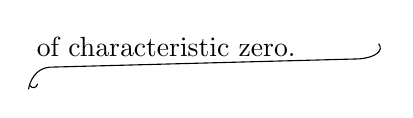
\begin{tikzpicture}[baseline=-.2ex,x=1em,y=1em]
\node[anchor=base west] at (0,.5) {of characteristic zero.};
\draw (.05,-.7) .. controls (.1,-.4) and (.3,.05) .. (.8,.1) -- (12,.4) .. controls (12.6,.45) and (12.9,.7) .. (12.7,.95);
\draw (.08,-.55) .. controls (.2,-.7) and (.35,-.65) .. (.38,-.5);
\end{tikzpicture}} To prove that, for the corresponding Galois group $G$ to be profinite, it is necessary and sufficient that for every object $M$ of $\underline{C}$, the $\otimes$-category generated be semisimple and have only a finite number of non-isomorphic simple objects. If $\underline{C}$ is arbitrary, the full subcategory \deleted{of} $\underline{C}_o$ of $\underline{C}$ which corresponds to the quotient pro-group of $G$ formed by the $\inserted{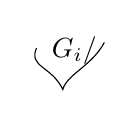
\begin{tikzpicture}[baseline=-.2ex,x=1em,y=1em]
\node[anchor=base west] at (0,.5) {$G_i\handwritten{/}$};
\draw (-.2,.85) .. controls (-.5,.15) and (.35,.2) .. (.75,-.65) .. controls (.9,-.1) and (1.8,.2) .. (2.25,1.05);
\end{tikzpicture}}G_i^o$ (where $G=\underset{\handwritten{\longleftarrow}}{\lim}G_i$, and $G_i^o$ is the identity component of $G_i$) is\rlap{\raisebox{-.9ex}{\tikz[x=1em,y=1em]{\fill (0,0)--(.12,.02)--(.08,.13)--cycle;\fill (.09,.2)--(.16,.28)--(.1,.36)--cycle;}}} made up exactly of the objects $M$ having the preceding property.

It would be interesting to find corresponding statements in arbitrary characteristic.

6) The notion of polarization of a motive over a field (itself deduced from that of polarization of an algebraic variety) gives a remarkable additional structure in the category of motives: if $M$ is a motive of weight $n$, one knows how to distinguish among the symmetric ($n$ even) resp. alternating ($n$ odd) forms $M\otimes M\handwritten{\rightharpoonup} T(n)$ (where $T$ is the Tate motive) those which are ``positive definite'' or again \handwritten{``}polarizations\handwritten{''}. This notion is reflected for example by additional structures on the motivic Galois groups. There is reason to make an abstract axiomatic study of such a notion of polarization on a general $\otimes$-category over a \deleted{field} subfield of the field of real numbers. We can discuss this again on occasion.\margin{\tikz[x=1em,y=1em]{\draw (0,0).. controls (.08,.02) and (.16,.14)..(.2,.28);}}
